\begin{figure}
  \centering
  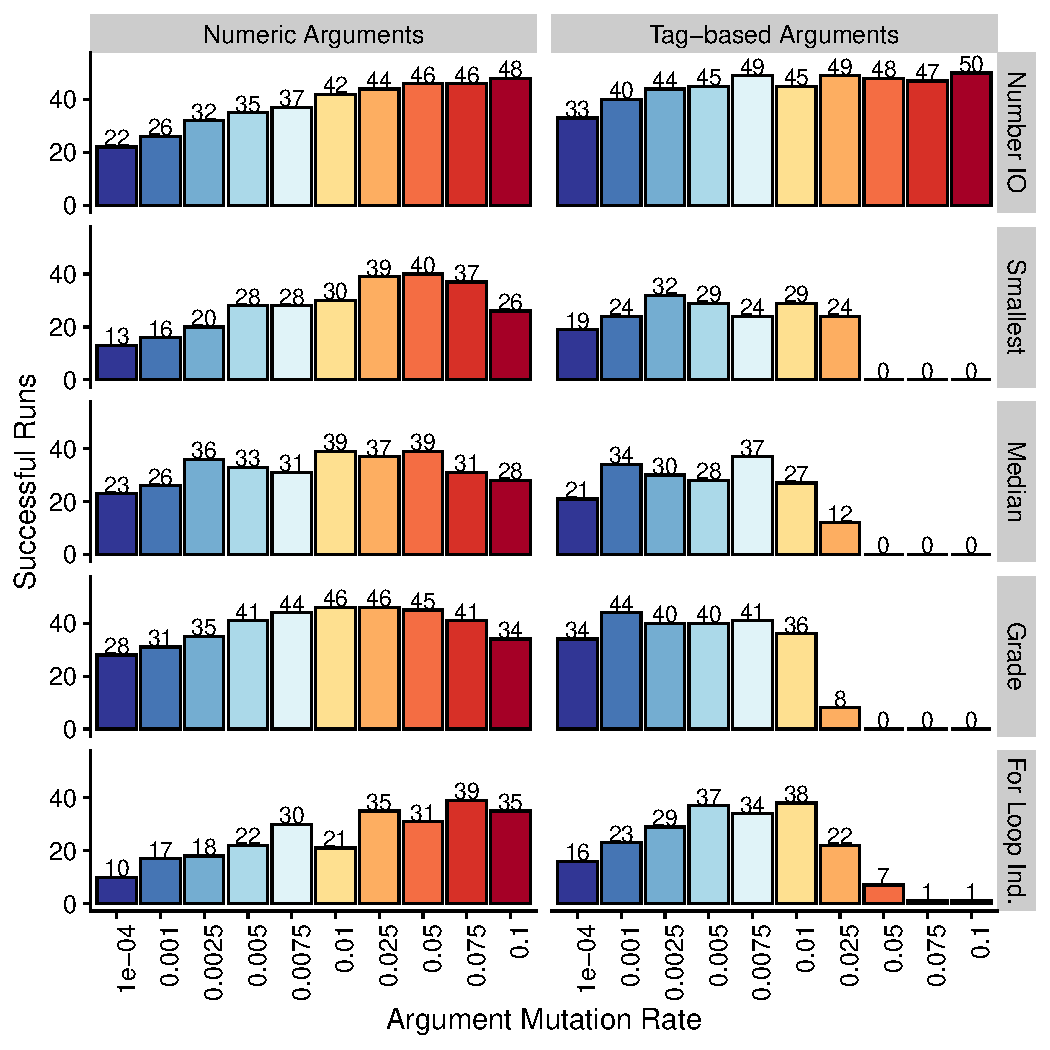
\includegraphics[width=0.75\columnwidth]{chapters/06-tag-access-memory/media/problem-solving-success.pdf}
  \caption{\small 
  \textbf{Number of successful runs} when using tag-accessed memory (right column) versus using traditional direct-indexed memory (left column) across five problems and ten instruction argument mutation rates (after 100 generations for number IO and 500 generations for all other problems).
  }
  \label{chapter:tag-accessed-memory:fig:successful-runs}
\end{figure}